\documentclass[11pt]{article}
\usepackage[a4paper,margin=26mm]{geometry}
\usepackage{amsmath,amssymb,amsthm,mathtools}
\usepackage{graphicx}
\usepackage{microtype}
\usepackage[hidelinks]{hyperref}
\usepackage{enumitem}

\newtheorem{theorem}{Theorem}
\newtheorem{corollary}[theorem]{Corollary}
\newtheorem{lemma}[theorem]{Lemma}
\newcommand{\C}{\mathbb C}
\newcommand{\Spec}{\operatorname{Spec}}

\title{A scattered-target criterion for compatible discretization\\
and faithful discretization of FDI $C^*$-algebras}
\author{Substantial partial result for arXiv:1607.03376}
\date{13 August 2026}

\begin{document}
\maketitle

\noindent\textbf{Status.}
Likely valid substantial partial result.  It gives new positive classes for
Question~2.6 of the source, but does not settle the question for arbitrary
$C^*$-algebras.

\section{Source question}

For a commutative unital $C^*$-algebra $C=C(X)$, write
$L(C)=\ell^\infty(X)$.  The source constructs a universal functorial
discretization
\[
 \eta_A:A\longrightarrow
 F(A)=\mathop{\operatorname{colim}}_{C\subseteq A\ \mathrm{commutative}}
       A*_{C}L(C).
\]
Question~2.6, on source PDF page~5, asks whether $\eta_A$ is injective or
faithful for every $A$, equivalently whether every $A$ has an injective or
faithful compatible $C^*$-discretization \cite{source}.

\begin{center}
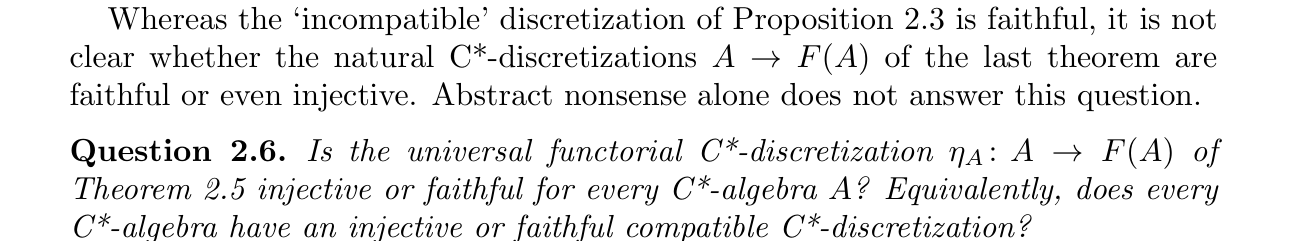
\includegraphics[width=\textwidth]{figures/question_2_6_crop.png}
\end{center}

All algebras and homomorphisms below are unital, as in the source.  We call a
$C^*$-algebra scattered when every commutative $C^*$-subalgebra has scattered
Gelfand spectrum.  We use the standard fact that, for a scattered compact space
$X$, every Radon measure is atomic and hence
\begin{equation}\label{eq:scattered-bidual}
 C(X)^{**}\cong \ell^\infty(X)
\end{equation}
canonically as von Neumann algebras.

\section{A general criterion}

\begin{theorem}[scattered-target criterion]\label{thm:criterion}
Let $A$ be a unital $C^*$-algebra and let
$\{\pi_i:A\to B_i\}_{i\in I}$ be unital $*$-homomorphisms into scattered
$C^*$-algebras.  Put $M=\prod_{i\in I}B_i^{**}$ and
\[
 \Phi:A\longrightarrow M,
 \qquad \Phi(a)=(\pi_i(a))_i.
\]
Then $\Phi$ has canonical normal context extensions
\[
 \Phi_C:\ell^\infty(\Spec C)\longrightarrow M
\]
that make it a compatible $W^*$-discretization.  Moreover:
\begin{enumerate}[label=\textup{(\roman*)}]
\item $\Phi$ is injective if and only if the family $(\pi_i)$ separates the
points of $A$;
\item $\Phi_C$ is injective if and only if
\begin{equation}\label{eq:coverage}
 \Spec C=\bigcup_{i\in I}
 r_{i,C}\bigl(\Spec(\pi_i(C))\bigr),
\end{equation}
where $r_{i,C}(y)=y\circ\pi_i|_C$.
\end{enumerate}
Consequently separation together with \eqref{eq:coverage} for every
commutative $C\subseteq A$ gives a faithful compatible $W^*$-discretization.
\end{theorem}

\begin{proof}
Fix a commutative $C\subseteq A$, set $X=\Spec C$ and
$Y_i=\Spec(\pi_i(C))$.  Since $\pi_i(C)$ is a commutative subalgebra of the
scattered algebra $B_i$, it is scattered.  Thus \eqref{eq:scattered-bidual}
identifies
\[
 \ell^\infty(Y_i)\cong \pi_i(C)^{**}.
\]
The quotient map $C\to\pi_i(C)$ is Gelfand dual to the injection
$r_{i,C}:Y_i\to X$.  Define the $i$th coordinate of $\Phi_C$ by
\begin{equation}\label{eq:coordinate}
 \ell^\infty(X)\xrightarrow{f\mapsto f\circ r_{i,C}}
 \ell^\infty(Y_i)\cong\pi_i(C)^{**}
 \xrightarrow{(\pi_i(C)\hookrightarrow B_i)^{**}}B_i^{**}.
\end{equation}
Every arrow is a normal unital $*$-homomorphism.  On $C=C(X)$ this is exactly
$\pi_i|_C$, so $\Phi_C$ extends $\Phi|_C$.

If $C\subseteq D$, the four spectral restriction maps satisfy
\[
 r_{i,C}\circ\bigl(\Spec(\pi_i(D))\to\Spec(\pi_i(C))\bigr)
 =\bigl(\Spec D\to\Spec C\bigr)\circ r_{i,D}.
\]
Pullback of bounded functions and bidual functoriality therefore show, one
coordinate at a time, that $\Phi_C$ factors through $\Phi_D$ by the source's
induced map $L(C)\to L(D)$.  This is compatibility.

Part (i) follows immediately from the product definition.  For (ii), the
kernel of the $i$th restriction in \eqref{eq:coordinate} consists of the
bounded functions vanishing on $r_{i,C}(Y_i)$.  Hence
\[
 \ker\Phi_C=\{f\in\ell^\infty(X):f=0\text{ on }
 \textstyle\bigcup_i r_{i,C}(Y_i)\}.
\]
This kernel is zero precisely when the union is all of $X$: if a point $x$ is
missing, its characteristic function $\delta_x$ is a nonzero kernel element.
\end{proof}

\section{Two positive classes}

\begin{corollary}[scattered algebras]\label{cor:scattered}
If $A$ is scattered, then $A\to A^{**}$ is a faithful compatible
$W^*$-discretization.  In particular, the source's universal
$\eta_A:A\to F(A)$ is faithful.
\end{corollary}

\begin{proof}
Apply Theorem~\ref{thm:criterion} to the singleton family
$\pi=\operatorname{id}_A$.  Separation and spectral coverage are tautological.
The last assertion follows from universality: the compatible discretization
factors as $A\xrightarrow{\eta_A}F(A)\to A^{**}$.  Likewise, each injective
context map factors through the corresponding canonical map
$L(C)\to F(A)$, forcing all those canonical maps, as well as $\eta_A$, to be
injective.
\end{proof}

Recall that an FDI algebra is one whose irreducible representations are all
finite-dimensional.  For unital algebras this is equivalent to being liminal,
or CCR: an irreducible image is $K(H)$, and its unit forces $H$ to be finite
dimensional.

\begin{corollary}[FDI/CCR algebras]\label{cor:fdi}
Every unital FDI (equivalently unital CCR) $C^*$-algebra has a faithful
compatible atomic $W^*$-discretization.  Consequently its universal map
$A\to F(A)$ is faithful.
\end{corollary}

\begin{proof}
Take one representative $\pi$ of every irreducible representation.  Its image
is a full matrix algebra, hence scattered, and irreducible representations
separate the points of $A$.

It remains to prove spectral coverage.  Let $C\subseteq A$ be commutative and
$x\in\Spec C$.  The pure state $x$ of $C$ has a pure-state extension $\omega$
to $A$.  Its GNS representation $(\pi_\omega,H_\omega,\xi_\omega)$ is
irreducible and therefore finite-dimensional.  For every $c\in C$,
\[
 \|\bigl(\pi_\omega(c)-x(c)\bigr)\xi_\omega\|^2
 =\omega\bigl((c-x(c))^*(c-x(c))\bigr)=0.
\]
Thus $\xi_\omega$ is a joint eigenvector for $\pi_\omega(C)$ with character
$x$.  Equivalently, $x$ belongs to the image of
$\Spec(\pi_\omega(C))\to\Spec C$.  Since $x$ was arbitrary,
\eqref{eq:coverage} holds.  Theorem~\ref{thm:criterion} and the same universal
factorization argument as in Corollary~\ref{cor:scattered} finish the proof.
\end{proof}

This genuinely exceeds the source's subhomogeneous result: the unital algebra
\[
 \left(\bigoplus_{n\ge1}^{c_0} C([0,1],M_n)\right)^{\!\sim}
\]
is FDI, but its irreducible dimensions are unbounded, so it is not
subhomogeneous.  It also has commutative subalgebras with non-scattered spectra,
so Corollaries~\ref{cor:scattered} and \ref{cor:fdi} provide distinct routes.

\section{Why the full question remains}

Eight focused attempts are recorded with the packet.  Two obstructions prevent
promotion to a full answer.

First, although every individual pushout $A*_C L(C)$ contains $A$ faithfully,
the compatibility colimit is indexed by the nonfiltered poset of commutative
contexts.  Context diamonds produce latching maps for which the iterated
amalgamated-free-product embedding argument used by the source's incompatible
construction does not apply.

Second, the source's relatively diffuse pairs force the atomic projections from
two context extensions to be mutually orthogonal.  In an AW*-target, arbitrary
projection suprema recover both units and give a contradiction.  An arbitrary
$C^*$-target has neither those suprema nor normality of maps out of
$\ell^\infty$, so the same argument does not force a nonzero element of $A$ into
the kernel.  Passing to the bidual does not repair this: the extended context
maps need not agree there as normal maps.

The successful criterion also has a sharp reach obstruction.  Simple purely
infinite algebras admit no nonzero maps into scattered algebras: a nonzero map
would be injective, while subalgebras of scattered algebras are scattered.
Thus a full solution requires an idea beyond scattered targets.

\section{Verification and novelty}

The accompanying finite-set script checks the contravariant spectral square,
the exact coverage criterion, and the missing-point characteristic-function
kernel witness.  These computations audit the combinatorial core; they do not
replace the operator-algebra proof.

A bounded novelty search on 12--13 August 2026 used arXiv:1607.03376, the exact
question wording, and combinations of ``universal functorial
$C^*$-discretization'', ``compatible'', ``FDI'', ``CCR'', ``liminal'', and
``scattered''.  It found the source and its earlier AW*-obstruction paper, but
no explicit statement of Theorem~\ref{thm:criterion} or
Corollary~\ref{cor:fdi}.  Novelty confidence is moderate pending expert citation
review.

\medskip
\noindent\textbf{Human-review recommendation.}
Check the normal identification \eqref{eq:scattered-bidual}, the spectral
naturality square used for compatibility, and the pure-state extension step in
Corollary~\ref{cor:fdi}.  These are the only substantive external standard
facts.

\begin{thebibliography}{9}
\bibitem{source}
C.~Heunen and M.~L. Reyes,
\emph{Discretization of $C^*$-algebras},
arXiv:1607.03376v2 (2017), Question~2.6, PDF p.~5.
\end{thebibliography}

\end{document}

